\documentclass{icga}
\usepackage{graphicx, epstopdf, amsmath, mathtools, amssymb, color, comment, mathabx, setspace, algorithm, fixltx2e, nicefrac, pgfplots, tikz, etoolbox, etex}
\usetikzlibrary{pgfplots.groupplots}
\pgfplotsset{compat=1.10}
\usepackage[algo2e, longend, noline, linesnumbered]{algorithm2e}

\SetKwIF{If}{ElseIf}{Else}{if}{then}{else if}{else}{endif}
\DeclarePairedDelimiter{\ceil}{\lceil}{\rceil}
\DeclarePairedDelimiter{\floor}{\lfloor}{\rfloor}
\DeclareMathOperator*{\argmax}{arg\,max}
\DontPrintSemicolon
\newcommand{\bE}{\mathbb{E}}
\newcommand{\eg}{{\it e.g.,}~}
\newcommand{\ie}{{\it i.e.,}~}
\newcommand{\cf}{{cf.}~}
\newcommand{\func}[1]{{\sc #1}}
\newcommand{\mctssr}{MCTS_{\mathcal{S}\mathcal{R}}}
\newcommand{\tuple}[1]{\ensuremath{\left \langle #1 \right \rangle }}
\newcommand{\TODO}[1]{\textbf{\color{red}#1}}
\newcommand\mycommfont[1]{\footnotesize\ttfamily{#1}}
\newcommand{\toexpand}[1]{{\it $\ll$ #1 ... $\gg$ }} 

\newcommand\NoIndent[1]{%
  \par\vbox{\parbox[t]{\linewidth}{#1}}%
}

\graphicspath{{img/}}
\DeclareGraphicsExtensions{.pdf,.jpg,.png,.eps}

\title{A Solver for Sequential Halving Applied to Trees}
\runningtitle{A Solver for Sequential Halving Applied to Trees}

\author{Tom~Pepels \and Mark~H.M.~Winands}

\author{Tom Pepels\thanks{e-mail:tom.pepels@maastrichtuniversity.nl} \and M.H.M. Winands\thanks{e-mail:m.winands@maastrichtuniversity.nl}}
\affiliation{Maastricht University, Maastricht, The Netherlands} \issue{?, ?}

\begin{document}
\maketitle
\begin{abstract}
In this paper, a solver is introduced for SHOT and Hybrid MCTS, allowing wins and losses to be proven in the tree. The solver is designed such that it does not disrupt the budget allocations of Sequential Halving. As such budget that is unspent when a proven node is encountered is spent during later rounds. The performance of the proposed enhancement is assessed in $n$ different two-player games: 
\end{abstract}

\section{Introduction}

\section{Sequential Halving Applied to Trees}
\label{sec:SHOT}

A recent addition to simple regret techniques in MCTS is Sequential Halving applied to Trees (SHOT)~\cite{Cazenave14SHOT}. The algorithm is presented as a ``faster'' version of MCTS. Instead of using UCT and backing up values after each simulation from leaf to root, SHOT uses Sequential Halving throughout the tree. This essentially turns MCTS into an iterative deepening, depth first search. The main benefit the author points out is that SHOT spends much less time in the tree, updating and back-propagating values. Consequently, an optimized engine with fast play-outs can perform more simulated games per turn using SHOT than it could with UCT. In practice it means that for the same number of play-outs SHOT is approximately twice as fast as UCT. SHOT allocates a
possibly large number of play-outs to the possible moves. This makes it quite easy to parallelize without loss of information and without changing the behaviour of the algorithm.

In the MAB context, Sequential Halving is run once, but in MCTS, nodes can be revisited, and therefore Sequential Halving is ``restarted'' upon revisiting a node. Define a \emph{cycle} as one full iteration of Sequential Halving which starts on line~\ref{shot:cycle}, and a \emph{round} as a sub-iteration over a given subset of $S$ which starts on line~\ref{shot:round}, in Algorithm~\ref{alg:shot}. Because any number of cycles may be started on a given node, care must be taken that budget is divided such that after any cycle the visit counts of all nodes are as if only one cycle was run. Therefore, when dividing the budget on line \ref{shot:budgeting} the current budget spent is added to the allocated budget, essentially overestimating the total budget available. Next, on line \ref{shot:topoff} only the budget that exceeds the current child's visits is allocated. This is illustrated in Figure \ref{fig:shot-topoffs}, where a node that was previously visited 64 times starts a new cycle with a budget of 128. The new budget per arm is: $\floor[\big]{\frac{64 + 128}{4\times\ceil{log_2{4}}}} = 24$. However, since the second and fourth child have previously been assigned a total budget of 24, only the first and third node are assigned $24-8=16$ budget.

\begin{figure}[ht]
	\centering
	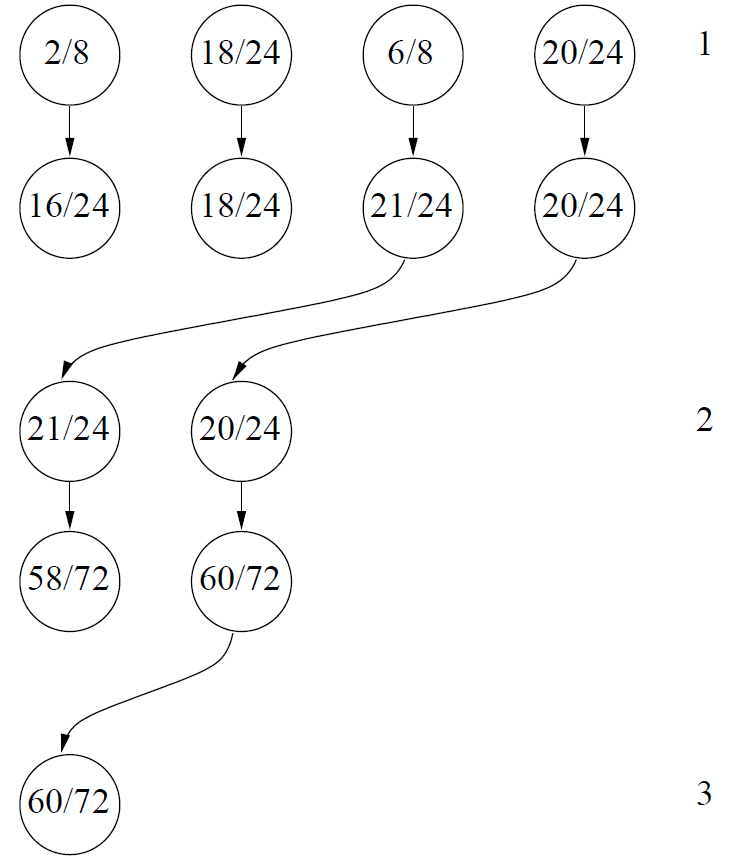
\includegraphics[width=.3\textwidth]{img/shot_topoffs.png}
	\caption{Division of 128 play-outs. The current node was previously visited 64 times~\cite{Cazenave14SHOT}.}
	\label{fig:shot-topoffs}
\end{figure}

SHOT was demonstrated to outperform UCT in NoGo, both on $9\times9$, and $19\times19$ boards, with win-rates between $75\%$ and $100\%$~\cite{Cazenave14SHOT}. However, based on the results in the article and Chapter \ref{chap:experiments}, these results were due to SHOT being significantly faster than UCT, when both algorithms are given the same budget of play-outs, different results are achieved.

Although in the original article SHOT is presented with the use of a transposition table instead of a tree, in Algorithm \ref{alg:shot} a version of SHOT using a tree of game states is presented.

\IncMargin{2em}
\RestyleAlgo{boxruled}
\begin{algorithm2e}[ht]
\setstretch{0.95}
	\KwIn{node $p$, allocated budget $budget$}
	\KwOut{tuple containing the number of visits, $p1$ and $p2$ wins, budget used}
	\func{shot}(node $p$, $budget$):													\;
	\Indp
	\lIf{isLeaf($p$)}{$S\gets$ \func{expand}($p$)}					
	$t_p \gets \tuple{0,0,0,0}$															\;
	\If{isTerminal($p$)}{																	\label{shot:terminal}
		\func{update} $t_p$, with $budget$ wins for the appropriate player and $budget$ visits 					\;
		\KwRet{$t_p$}																	\;
	}
	\If{budget = 1} {																		\label{shot:playout}
		$r \gets$ \func{playout}($p$)													\;
		\func{update} $t_p$, with 1 budget used, 1 win for the appropriate player, and 1 visits					\;
		\KwRet{$t_p$}																	\;
	}
	\If{$|S|$ = 1} {
		$n_0 \gets$ the single element in $S$											\;
		$t_p \gets $ \func{shot}($n_0$, $budget$)											\;
		\func{update} $p$ with $t_p$													\;
		\KwRet{$t_p$}																	\;	
	}
	$s \gets |S|$, $S_0 \gets S$, $b_u, b, k \gets 0$									\;
	\While{$s >$ 1 \textbf{and} $b_u < budget$} {											\label{shot:cycle}
	$b \gets b + \displaystyle\max{\left(1, \floor[\bigg]{\frac{p.budgetSpent + budget}{s\times\ceil{log_2{|S|}}}}\right)}$ \;	\label{shot:budgeting}
		\For{i=1 \emph{\KwTo} s}{															\label{shot:round}
			$n_i \gets$ node $n$ at rank $i$ of $S_k$									\;
			$b_i \gets b - n_i.visits$													\;  \label{shot:topoff}
			\If{$b_i > 0$} {
				\If{$p$ is root \textbf{and} $i = 0$ \textbf{and} $s = 2$} {
					$b_i \gets \max{(b_i, budget - b_u - (b - n_1.visits))}$				\;
				}
				$b_i \gets \min{(b_i, budget - b_u)}$										\;
				$\tuple{v, w_1, w_2, b_{u, n_i}}_i \gets$ \func{shot}($n_i$, $b_i$)			\;
				\func{update} $p, b_u,$ and $t_p$ with $\tuple{v, w_1, w_2, b_{u, n_i}}_i$	\; \label{shot:tp_update}
			}
			break if $b_u \geq budget$													\;
		}
		$k \gets k + 1$																		\;
		$S_{k} \gets$ $S_{k-1}$ sorted in descending order									\;
		$s \gets \ceil{\nicefrac{s}{2}}$													\;
	}
	\func{update} $p.budgetSpent$ with $b_u$												\; \label{shot:budg_spent}
	\Indm
	\KwRet{$t_p$}
  \caption{Sequential Halving applied to Trees (SHOT)~\cite{Cazenave14SHOT}. \label{alg:shot}}
\end{algorithm2e}
\DecMargin{2em}

SHOT recursively performs Sequential Halving until either a terminal state is encountered (line \ref{shot:terminal}), or the available budget for the current node is 1 (line \ref{shot:playout}). Because multiple play-outs can be performed from a single recursive call, a tuple $t_p$ is maintained containing: 1) the budget used $b_u$, 2) the number of wins per player $w_1$ and $w_2$, and 3) the number of visits $v$. $v$ differs from $b_u$, because visiting a terminal node spends no budget, but performing a play-out does, and in both cases the visit count of the node should be increased. On line~\ref{shot:tp_update}, $p$ is updated with the results returned from the recursion, $b_u$ is updated with the total budget used by play-outs, and $t_p$ is updated with all returned values. On line~\ref{shot:budg_spent} the total budget spent at the current node is incremented. This value is used to determine the budget of the next round of SHOT.

A disadvantage of SHOT is that it cannot be terminated any time, and requires a-priori knowledge of the available budget. The pure exploration policies discussed in Chapter \ref{chap:mab} guarantee a low simple regret on the recommendation only after all available $T$ simulations are performed. Therefore, they cannot be terminated, or asked for a reasonable recommendation before this limit is reached.

This leads to another concern when using any pure exploration policy recursively. As discussed in Chapter \ref{chap:mab}, UCT has the advantage of almost exclusively selecting the best node over time, giving the formal guarantee that suboptimal nodes are selected at most $O(\ln{n})$ times. This ensures that over time, values accumulated at nodes approximate the value of the best-reply to the node's move. With a policy such as Sequential Halving this guarantee is related to the available budget and the branching factor. In fact, the two empirically best nodes are sampled equally, however different their reward may be. Moreover, for a node with a set of children $S$, the worst $\frac{|S|}{2}$ of these are sampled at least at total of $\floor{\frac{T}{\ceil{log_2{|S|}}}}$ times. In many games there are only a handful of good moves given a position, and to evaluate a node the value of its move's best-reply must be found. By using Sequential Halving throughout the tree, values back-propagated do not converge in the same manner as UCT, as such, values of internal nodes are constituted of more overall averages over their children.

\section{A Solver for SHOT}
\label{sec:shotsolver}

In the form presented in Algorithm~\ref{alg:shot}, SHOT cannot solve proven wins or losses in the simple regret tree. A solver for UCT was previously proposed by Winands et al.~\citeaby{Winands2008}, named MCTS-Solver. However, this technique requires adaptation for Sequential Halving to be able to solve nodes in SHOT. The main issue here is that when a solved child is encountered, the current round is interrupted to determine whether the node itself is solved as well. This leads to the following three different possible cases in which this interruption can be encountered. In each case, it is assumed that values are represented according to negamax, such that at each node, children's rewards are stored with respect to the player to move.
\begin{enumerate}
\item A solved win is encountered, in this case, we immediately want to remember this node and back-propagate to the parent. Any residual budget remains unspent in the current round.
\item A solved loss is encountered, but not all siblings lead to a loss. According to~\citeaby{Winands2008} it is appropriate in this case to count the visit as a loss. However, since there still exist nodes that do not lead to a loss, we have to ensure the solved node is not reselected. If it is reselected, a potentially high budget may be spent on the node, which results in an underestimation of the parent.
\item A solved loss is encountered, and all siblings lead to a loss. In this case the parent is a win and we should back-propagate immediately. Any residual budget remains unspent in the current round.
\end{enumerate}
\begin{figure}[ht]
	\centering
	\includegraphics[width=.6\textwidth]{img/solver.png}
	\caption[SHOT Solver example]{SHOT Solver removing a proven loss from selection. In the second round, node B is determined to be a proven loss, node C is returned to selection to fill the empty position.}
	\label{fig:shot_solver}
\end{figure}

When running Sequential Halving, the first and last cases can be handled similar to the MCTS-Solver. The second case potentially leaves the assigned budget partially unspent. Because some children have been identified as a loss, while other unsolved options still remain, the proven losses should be removed from selection. Moreover, any budget left unspent due to this should be ``brought over'' to the next round, which starts with a reduced set of nodes. When a proven loss is discarded from selection, all children following this node move one position left, possibly returning an unsolved node to the current selection, as depicted in Figure~\ref{fig:shot_solver}. If there is no unsolved node to return, then the set of remaining arms is reduced after the round if it is smaller than $\ceil{\nicefrac{s}{2}}$, which means that more than half the nodes currently in $S_k$ were solved.

\IncMargin{2em}
\RestyleAlgo{boxruled}
\begin{algorithm2e}[ht]
\setstretch{0.95}
	\KwIn{node $p$, allocated budget $budget$}
	\KwOut{tuple containing the number of visits, $p1$ and $p2$ wins, budget used}
	\func{shot}(node $p$, $budget$):													\;
	\Indp
	\lIf{isLeaf($p$)}{$I, S\gets$ \func{expand}($p$)}								\label{ss:children}		
	$t_p \gets \tuple{0,0,0,0}$															\;
	\If{isTerminal($p$)}{																	
		\func{update} $t_p$, with $budget$ wins for the appropriate player and $budget$ visits 					\;
		\KwRet{$t_p$}																	\;
	}
	\If{budget = 1} {																		
		$r \gets$ \func{playout}($p$)													\;
		\func{update} $t_p$, with 1 budget used, 1 win for the appropriate player, and 1 visits					\;
		\KwRet{$t_p$}																	\;
	}
	\If{$|S|$ = 1} {
		$n_0 \gets$ the single element in $S$											\;
		$t_p \gets $ \func{shot}($n_0$, $budget$)											\;
		\func{update} $p$ with $t_p$													\;
		\KwRet{$t_p$}																	\;	
	}
	$s \gets |S|$, $S_0 \gets S$, $b_u, k \gets 0$									\;
	$b \gets b + \displaystyle\max{\left(1, \floor[\bigg]{\frac{p.budgetSpent + budget}{s\times\ceil{log_2{|S|}}}}\right)}$ \;
	\While{$s >$ 1 \textbf{and} $b_u < budget$} {										
	$b_r \gets 0$ 																		\; \label{ss:resid}
		\For{i=1 \emph{\KwTo} s}{
			$n_i \gets$ node $n$ at rank $i$ of $S_k$									\;
			\If{$n_i$ is not solved} {
				$b_i \gets b - n_i.visits$													\;  
				\If{$b_i > 0$} {
					\If{$p$ is root \textbf{and} $i = 0$ \textbf{and} $s = 2$} {
						$b_i \gets \max{(b_i, budget - b_u - (b - n_1.visits))}$				\;
					}
					$b_i \gets \min{(b_i, budget - b_u)}$										\;
					$\tuple{v, w_1, w_2, b_{u, n_i}}_i \gets$ \func{shot}($n_i$, $b_i$)			\;
					\func{update} $p, b_u,$ and $t_p$ with $\tuple{v, w_1, w_2, b_{u, n_i}}_i$	\;
				}
			}
			\uIf{$n_i$ is a win \textbf{or} $(n_i$ is a loss \textbf{and} $\forall n \in S: (n$ is a loss$))$}{
				set the solved player in $t_p$												\; \label{ss:solved}
				\func{update} $p.budgetSpent$ with $b_u$									\;
				\KwRet{$t_p$}																\;
			} \ElseIf{$(n_i$ is a loss \textbf{and} $\exists n \in S: (n$ is not a loss$))$} {
				$b_r \gets b_i - v$															\; \label{ss:update_resid}				
			}
			break if $b_u \geq budget$														\;
		}
		remove all solved nodes from $S$ and $S_k$											\;  \label{ss:remove}
		$k \gets k + 1$																		\;
		$S_{k} \gets$ $S_{k-1}$, with the first $\max{(2, s)}$ elements sorted in descending order \; \label{ss:sort}
		$s \gets \min{(\ceil{\nicefrac{s}{2}}, |S|)}$										\; \label{ss:size_min}	
		\lIf{$s = 1$} {$b \gets b + (budget - b_u)$}
		\Else {	
			$b \gets b + \ceil{\nicefrac{b_r}{s}} + \max{\left(1, \floor[\bigg]{\frac{p.budgetSpent + budget}{s\times\ceil{log_2{|S|}}}}\right)}$ \; \label{ss:incr_budget_resid}
		}
	}
	\func{update} $p.budgetSpent$ with $b_u$												\;
	\Indm
	\KwRet{$t_p$}
  \caption{SHOT Solver. \label{alg:shot-solver}}
\end{algorithm2e}
\DecMargin{2em}

SHOT Solver is outlined in Algorithm~\ref{alg:shot-solver}. The general procedure when a solved node is encountered is straightforward in the case of a solved win, and when all children are solved losses. The $budgetSpent$ is updated and the function immediately returns. The tuple $t_p$ now also contains a `solved' field, which holds the index of the player for which the node is solved. In this case the \func{update} function updates the node accordingly by setting the $isSolved$ flag. When an isolated proven loss is encountered, \ie not all siblings are losses, then we should not sample that node again, since it would under-evaluate the parent. This possibly leaves a residual budget $b_r$ declared on line~\ref{ss:resid}, which is maintained per round. When an isolated proven loss is found, the residual budget is updated on line~\ref{ss:update_resid} such that it can be spent in the next round with a reduced set of nodes, on line~\ref{ss:incr_budget_resid}. Moreover, since the isolated losses are removed from $S$ on line~\ref{ss:remove}, it is possible that $s > |S|$, which is restored on line~\ref{ss:size_min} after halving $s$. This ensures that previously removed nodes that were not proven losses can be returned to selection in case more than half of the nodes were solved in this round. On line~\ref{ss:sort} the set of children from the previous round $S_{k-1}$ is sorted, as such $|S_k| = |S|$ for each round. Therefore, when a solved loss is removed from selection, another child can take its place. Note also that on line~\ref{ss:children}, a second set $I$ contains all children. Because it is possible to remove all nodes from $S$ in case of a proven loss, $I$ is never altered and can be used to give a recommendation at the root.

\section{Experiments and Results}
\label{sec:experiments}
In this section, the influence of the solver enhancement in H-MCTS and SHOT is investigated. Experiments are performed to show the performance of the solver per technique individually, and for H-MCTS and SHOT against UCT.

\subsection{Experimental Setup}
\label{subsec:ex_setup}
In this chapter the results of the experiments performed on six two-player games are presented. H-MCTS and the games were implemented in two different engines. Amazons, Breakthrough, NoGo, and Pentalath are implemented in a Java based engine. Ataxx and AtariGo are implemented in a \emph{C++} based engine.\footnote{Experiments in Ataxx and AtariGo were performed in collaboration with Prof. Dr. Tristan Cazenave.} Whereas the former is a full implementation of SHOT, H-MCTS, H-MCTS Solver, and the Upper/Lower Bounds enhancement, the latter consists of an implementation of SHOT and H-MCTS.

A brief description of each game is given below:
\begin{itemize}
\item \emph{Amazons} is played on a 10$\times$10 chessboard. Players each have four Amazons that move as queens in chess. Moves consist of two parts, movement, and shooting an arrow to block a square on the board. The last player to move wins the game.
\item \emph{AtariGo}, or first-capture Go, is a variant of Go where the first player to capture any stones wins. The experiments are performed on a 9$\times$9 board.
\item \emph{Ataxx} is a game similar to Reversi. Played on a square board, players start with two stones each placed in an opposite corner. Captures are performed by moving a stone alongside an opponent's on the board. In the variant used in this thesis, jumps are not allowed. The game ends when all squares are filled, or when a player has no remaining stones. The player with the most stones wins.  The experiments are performed on a 7$\times$7 board.
\item \emph{Breakthrough} is played on an 8$\times$8 board. Players start with 16 pawns. The goal is to move one of them to the opponent's side.
\item \emph{NoGo} is a combinatorial game based on Go. Captures are forbidden and the first player unable to play due to this rule, loses. The experiments are performed on a 9$\times$9 board.
\item \emph{Pentalath} is a connection game played on a hexagonal board. The goal is to place 5 pieces in a row. Pieces can be captured by fully surrounding an opponent's set of pieces.
\end{itemize}

All games use a uniform random selection policy during the play-outs, unless otherwise stated. All algorithms use transposition tables to store the values of game-states, these tables are cleared between moves, such that no information is retained. The $C$ constant, used by UCT (Equation \ref{eq:uct}) was optimized for each game and was not re-optimized for H-MCTS, unless mentioned otherwise, both UCT and H-MCTS use the same $C$ constant. Table~\ref{tab:uct_c} lists the $C$ constant used by UCT and H-MCTS in the experiments in this section.

\subsection{Results}
\label{subsec:results}
For the tables and graphs in this subsection, results are shown with respect to the first algorithm mentioned in the captions, along with a 95\% confidence interval. For each experiment, the players' seats were swapped such that 50\% of the games are played as the first player, and 50\% as the second, to ensure no first-player or second-player bias.

\begin{figure}[h]
\centering
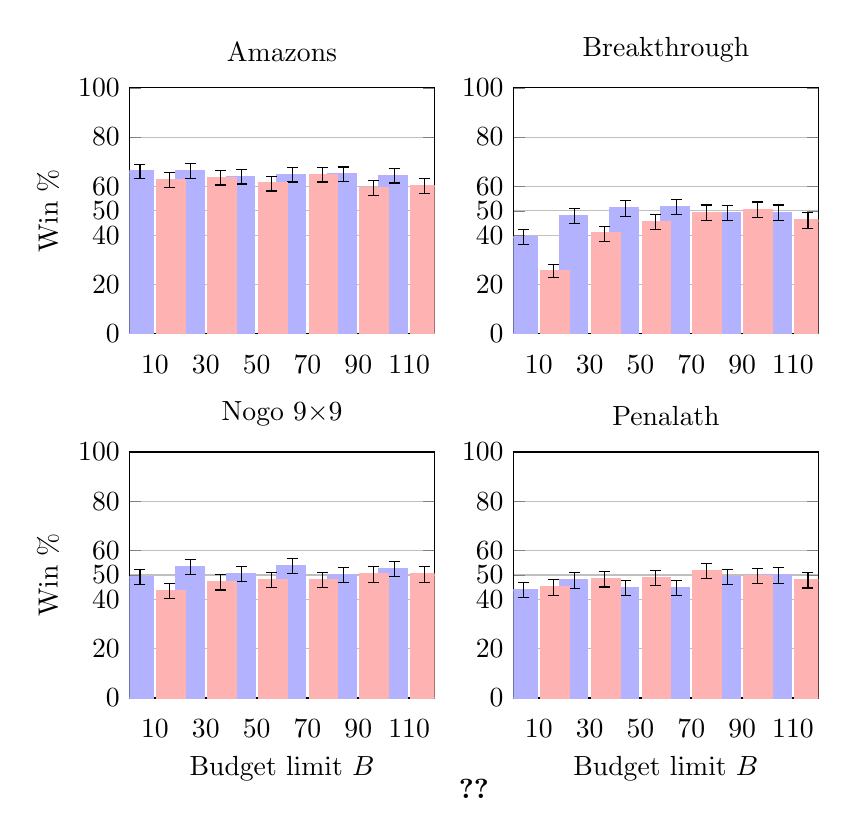
\begin{tikzpicture}
\begin{groupplot}
    [
        group style=
            {
            columns=2,
            rows=2,
            xlabels at=edge bottom,
            ylabels at=edge left,
            vertical sep= 1.5cm,
            },
       	width  = 0.45*\textwidth,
        major x tick style = transparent,
        ybar= 2 * \pgflinewidth,
        % bar width = 10pt,
        ymajorgrids = true,
        ylabel = {Win \%},
        xlabel= {Budget limit $B$},
        symbolic x coords={10,30,50,70,90,110},
        xtick = data,
        ytick={0,20,40,50, 60,80,100},
        scaled y ticks = false,
        enlarge x limits = 0.1,
        ymin=0,
        ymax=100,
    ]
% Amazons ----------------------------------------
\nextgroupplot[title=Amazons]
\addplot[blue!30!white, fill=blue!30!white, thick, error bars/.cd,
            y dir=both, error bar style={black},
            y explicit]
	coordinates {
	(10, 66) +- (0,2.94) 
	(30,66.2) +- (0,2.93)
	(50,63.9) +- (0,2.98)
	(70,64.7) +- (0,2.96)
	(90,64.9) +- (0,2.96)
	(110,64.3) +- (0,2.97)};
\addplot[red!30!white, fill=red!30!white, thick, error bars/.cd,
            y dir=both, error bar style={black},
            y explicit]
	coordinates {
	(10,62.6) +- (0,3)
	(30,63.5) +- (0,2.99)
	(50,61.1) +- (0,3.02)
	(70,64.7) +- (0,2.96)
	(90,59.3) +- (0,3.04)
	(110,60.1)+- (0,3.04)};
% Breakthrough -------------------------------------
\nextgroupplot[title=Breakthrough]
\addplot[blue!30!white, fill=blue!30!white, thick, error bars/.cd,
            y dir=both, error bar style={black},
            y explicit]
	coordinates {
	(10, 39.48) +- (0,3.03) 
	(30,47.8) +- (0,3.1)
	(50,50.95) +- (0,3.1)
	(70,51.6) +- (0,3.1)
	(90,49.2) +- (0,3.1)
	(110,49.3) +- (0,3.1)};
\addplot[red!30!white, fill=red!30!white, thick, error bars/.cd,
            y dir=both, error bar style={black},
            y explicit]
	coordinates {
	(10,25.45) +- (0,2.7)
	(30,40.78) +- (0,3.05)
	(50,45.35) +- (0,3.09)
	(70,49.3) +- (0,3.1)
	(90,50.5) +- (0,3.1)
	(110,46.1)+- (0,3.09)};
% Nogo --------------------------------------------
\nextgroupplot[title=Nogo 9$\times$9]
\addplot[blue!30!white, fill=blue!30!white, thick, error bars/.cd,
            y dir=both, error bar style={black},
            y explicit]
	coordinates {
	(10, 49.3) +- (0,3.1) 
	(30,53.3) +- (0,3.09)
	(50,50.4) +- (0,3.1)
	(70,53.6) +- (0,3.09)
	(90,50.0) +- (0,3.1)
	(110,52.5) +- (0,3.1)};
\addplot[red!30!white, fill=red!30!white, thick, error bars/.cd,
            y dir=both, error bar style={black},
            y explicit]
	coordinates {
	(10,43.6) +- (0,3.07)
	(30,47) +- (0,3.09)
	(50,48) +- (0,3.1)
	(70,48) +- (0,3.1)
	(90,50.2) +- (0,3.1)
	(110,50.2)+- (0,3.1)};

% Pentalath --------------------------------------------
\nextgroupplot[title=Penalath, legend to name=grouplegend2]
\addplot[blue!30!white, fill=blue!30!white, thick, error bars/.cd,
            y dir=both, error bar style={black},
            y explicit]
	coordinates {
	(10,44.04) +- (0,3.08) 
	(30,47.75) +- (0,3.1)
	(50,44.64) +- (0,3.08)
	(70,44.63) +- (0,3.09)
	(90,49.2) +- (0,3.1)
	(110,49.79) +- (0,3.1)};
	\addlegendentry{10,000 play-outs}
\addplot[red!30!white, fill=red!30!white, thick, error bars/.cd,
            y dir=both, error bar style={black},
            y explicit]
	coordinates {
	(10,44.96) +- (0,3.1)
	(30,48.24) +- (0,3.1)
	(50,48.75) +- (0,3.1)
	(70,51.75) +- (0,3.1)
	(90,49.6) +- (0,3.1)
	(110,47.84)+- (0,3.1)};
	\addlegendentry{25,000 play-outs}
\end{groupplot}

    \node (legend) at ($(group c1r2.south)!0.5!(group c2r2.south)$)
      [below, yshift=-2\pgfkeysvalueof{/pgfplots/every axis title shift}]
      {\ref{grouplegend2}};

\end{tikzpicture}
     \caption{H-MCTS Solver vs. MCTS-Solver with random play-outs. Win percentages with respect to H-MCTS, error bars represent 95\% c.i..}
     \label{fig:h-mcts-s_v_mcts-s}
\end{figure}



In Figure~\ref{fig:h-mcts-s_v_mcts-s} results are shown for different $B$ values for H-MCTS Solver. All games were played against the MCTS-Solver. As in Subsection~\ref{subsec:hmcts_uct}, the largest increases in performance are shown in Amazons and Pentalath. Breakthrough and NoGo both show positive results when the total budget is small, the benefit of H-MCTS decreases when the allocated budget increases. This is also visible in the best values for $B$, which are high for both games, implying that UCT is the preferred selection policy.

\begin{table}[ht]
\centering
\tabcolsep=0.3cm
\scalebox{0.95}{
\begin{tabular}{rlcc}
\hline
\multicolumn{2}{c|}{} & \multicolumn{1}{c}{\textbf{10,000}} & \multicolumn{1}{c}{\textbf{25,000}} \\ 
\textbf{Game} & \multicolumn{1}{c|}{} & \multicolumn{1}{c}{\textbf{play-outs}} & \multicolumn{1}{c}{\textbf{play-outs}} \\ [1mm] 
\cline{1-4}
\multicolumn{2}{c|}{} \\ [-3mm]
\multicolumn{2}{c|}{} & \multicolumn{2}{c}{\textbf{MCTS (UCT) Solver}} 												\\ [1mm]
\multicolumn{2}{c|}{} \\ [-4mm]
Amazons &\multicolumn{1}{l|}{}			    	& 50.2 $\pm$ 3.1 				& 50.6 $\pm$ 3.1 					\\ [.5mm] 
Breakthrough 8$\times$8 &\multicolumn{1}{l|}{}	& {\bf{53.7}} $\pm$ 3.1			& 49.0 $\pm$ 3.1 					\\ [.5mm] 
NoGo 9$\times$9 &\multicolumn{1}{l|}{} 			& 49.9 $\pm$ 2.2				& 49.9 $\pm$ 3.1 					\\ [.5mm] 
Pentalath &\multicolumn{1}{l|}{} 		  		& {\bf{53.7}} $\pm$ 3.1			& 48.6 $\pm$ 3.1 					\\ [.5mm] 
\multicolumn{2}{c|}{} \\ [-4mm]
\cline{1-4}
\multicolumn{2}{c|}{} \\ [-3mm]
\multicolumn{1}{c}{} & \multicolumn{1}{c|}{\textbf{$B$}} & \multicolumn{2}{c}{\textbf{H-MCTS Solver}} 				\\ [1mm]
\multicolumn{2}{c|}{} \\ [-4mm]
Amazons &\multicolumn{1}{l|}{90}			    	& 50.1 $\pm$ 3.1 				& 50.6 $\pm$ 3.1 				\\ [.5mm] 
Breakthrough 8$\times$8 &\multicolumn{1}{l|}{50}	& 52.8 $\pm$ 3.1				& 48.4 $\pm$ 3.1 				\\ [.5mm] 
NoGo 9$\times$9 &\multicolumn{1}{l|}{110} 			& 50.3 $\pm$ 3.1				& 48.3 $\pm$ 3.1 				\\ [.5mm] 
Pentalath &\multicolumn{1}{l|}{90} 		  			& {\bf{55.3}} $\pm$ 3.1			& 52.4 $\pm$ 3.1				\\ [.5mm] 
\multicolumn{2}{c|}{} \\ [-4mm]
\cline{1-4}
\multicolumn{2}{c|}{} \\ [-3mm]
\multicolumn{2}{c|}{} & \multicolumn{2}{c}{\textbf{SHOT Solver}} 													\\ [1mm]
\multicolumn{2}{c|}{} \\ [-4mm]
Amazons &\multicolumn{1}{l|}{}			    	& 49.6 $\pm$ 3.1 				& 49.4 $\pm$ 3.1 					\\ [.5mm] 
Breakthrough 8$\times$8 &\multicolumn{1}{l|}{}	& {\bf{53.8}} $\pm$ 3.1			& {\bf{53.4}} $\pm$ 3.1 			\\ [.5mm] 
NoGo 9$\times$9 &\multicolumn{1}{l|}{} 			& 50.1 $\pm$ 3.1				& 51.3 $\pm$ 3.1 					\\ [.5mm] 
Pentalath &\multicolumn{1}{l|}{} 		  		& {\bf{60.4}} $\pm$ 3.0			& {\bf{70.5}} $\pm$ 2.8 			\\ [.5mm] 
\hline
\end{tabular}
}
\vspace{3mm}
{\caption[H-MCTS, SHOT, and UCT with and without solver.]
{UCT, H-MCTS, and SHOT with and without solver, random play-outs. \\ Win percentages for the players with the solver enabled, 1,000 games.} \label{tab:solver_no_solver}}
\end{table}

The implementation of the solver was validated empirically, by comparing the performance of UCT, H-MCTS, and SHOT against themselves with the solver enhancement enabled. The results of this experiment are shown in Table~\ref{tab:solver_no_solver}. For H-MCTS without the solver enhancement, the $B$ values used in Subsection~\ref{subsec:shot_uct} were applied, the $B$ values presented in the table are those obtained from the results shown in Figure~\ref{fig:h-mcts-s_v_mcts-s}, this ensues both versions of the algorithm use a reasonable value for $B$.

The use of a solver has the most influence in Pentalath and Breakthrough. In Amazons and NoGo, games are mostly decided at the start, or in the middle of the game, meaning that the added benefit of discovering solved nodes near the end adds little to the overall performance. Although the solver did not result in a significant performance increase in most cases, it is possible that longer search-times and the use of heuristic play-outs results in an increase in performance overall.

Notably, the SHOT solver achieves a significantly high performance increase in both experimental cases in Pentalath. In Pentalath, all unoccupied positions can be played at any time, meaning that at each ply, excluding rarely occurring suicide moves, $o_p-1$ positions can be played where $o_p$ is the number of unoccupied positions at the parent. This also means that if any position results in a direct win for a player, it does so via multiple paths in the tree, which consequently results in almost all children of the root achieving a high value. Because of this, the algorithm does not recommend moves that will let it win fast, but possibly postpones its victory allowing its opponent to strengthen his position. In this case, the solver makes sure that when a solved node is found, it is excluded from normal search and immediately back-propagated, \ie when a solved position is found it is immediately played, instead of continuously searching for similarly good options.

\begin{table}[ht]
\centering
\tabcolsep=0.3cm
\scalebox{1.0}{
\begin{tabular}{rlll}
\hline
\multicolumn{2}{c|}{} & \multicolumn{1}{c}{\textbf{10,000}} & \multicolumn{1}{c}{\textbf{25,000}} \\ 
\textbf{Game} & \multicolumn{1}{c|}{\textbf{$B$}} & \multicolumn{1}{c}{\textbf{play-outs}} & \multicolumn{1}{c}{\textbf{play-outs}} \\ [1mm] 
\cline{1-4}
\multicolumn{2}{c|}{} \\ [-3mm]
Amazons &\multicolumn{1}{l|}{90}			    	& {\bf{64.9}} $\pm$ 2.1				& {\bf{62.5}} $\pm$ 2.1 		\\ [.5mm] 
Breakthrough 8$\times$8 &\multicolumn{1}{l|}{50}	& {\bf{54.5}} $\pm$ 2.2				& 48.4 $\pm$ 2.2 				\\ [.5mm] 
NoGo 9$\times$9 &\multicolumn{1}{l|}{110} 			& 49.6 $\pm$ 2.2					& 46.8 $\pm$ 2.2 				\\ [.5mm] 
Pentalath &\multicolumn{1}{l|}{90} 		  			& 50.8 $\pm$ 2.2					& {\bf{53.5}} $\pm$ 2.2 		\\ [.5mm] 
\hline
\end{tabular}
}
\vspace{3mm}
{\caption[H-MCTS Solver vs. MCTS-Solver.]{H-MCTS Solver vs. MCTS-Solver, random play-outs.\\ Win percentages with respect to H-MCTS, 2,000 games.} \label{tab:uct-s_hmcts-s}}
\end{table}

Table~\ref{tab:uct-s_hmcts-s} shows the results for games played with the solver enabled in both H-MCTS and UCT. Unlike Table~\ref{tab:uct_hmcts} there is a significant performance increase in four cases when the solver is enabled. It is likely that the increased exploration performed by SHOT is responsible for finding solved nodes faster, or in parts of the tree that UCT is less likely to visit. Similar to the results for H-MCTS against UCT in Table~\ref{tab:uct_hmcts}, the results give evidence that a higher number of play-outs give increasingly better results in Pentalath. To validate this conjecture an additional experiment was run with a budget of 50,000 play-outs, which resulted in a win-rate for H-MCTS of {\bf{55.7}}\%$\pm$3.1, another significant increase in performance over UCT.

\begin{table}[ht]
\centering
\tabcolsep=0.3cm
\scalebox{1.0}{
\begin{tabular}{rlcc}
\hline
\multicolumn{2}{c|}{} & \multicolumn{1}{c}{\textbf{10,000}} & \multicolumn{1}{c}{\textbf{25,000}} \\ 
\textbf{Game} & \multicolumn{1}{c|}{\textbf{$B$}} & \multicolumn{1}{c}{\textbf{play-outs}} & \multicolumn{1}{c}{\textbf{play-outs}} \\ [1mm] 
\cline{1-4}
\multicolumn{2}{c|}{} \\ [-3mm]
\multicolumn{2}{c|}{} & \multicolumn{2}{c}{\textbf{Heuristic play-outs (no solver)}} \\ [1mm]
\multicolumn{2}{c|}{} \\ [-4mm]
Breakthrough 8$\times$8 &\multicolumn{1}{l|}{70}	& 50.9 $\pm$ 3.1				& {\bf{56.6}} $\pm$ 3.1 	\\ [.5mm]
\multicolumn{2}{c|}{} \\ [-4mm]
\cline{1-4}
\multicolumn{2}{c|}{} \\ [-3mm]
\multicolumn{2}{c|}{} & \multicolumn{2}{c}{\textbf{Heuristic play-outs \& solver}} 					\\ [1mm]
\multicolumn{2}{c|}{} \\ [-4mm]
Breakthrough 8$\times$8 &\multicolumn{1}{l|}{70}	& {\bf{56.7}} $\pm$ 3.1		& {\bf{61.3}} $\pm$ 3.0 	\\ [.5mm]
\hline
\end{tabular}}
\vspace{3mm}
{\caption[H-MCTS vs. UCT, heuristic play-outs and solver.]{H-MCTS vs. UCT, heuristic play-outs, with/without solver.\\ Win percentages with respect to H-MCTS, 1,000 games} \label{tab:uct_hmcts-s-h}}
\end{table}

A heuristic play-out policy was developed for Breakthrough, it selects moves during play-out over a non-uniform distribution based on the properties of the moves. A capture move is four times more likely to be selected than a non-capture one, and a defensive capture (near the winning line) is five times more likely to be selected. Moreover, (anti-)decisive~\cite{teytaud2010huge} moves are always played when available. UCT with this play-out policy enabled wins approximately 78\% of the games played against UCT with random play-outs. 

For the results in Table~\ref{tab:uct_hmcts-s-h}, the informed play-out policy is used to select moves for Breakthrough. H-MCTS benefits more from the informed play-outs than UCT in Breakthrough, both when the solver is disabled, and even more so when it is enabled. This may be due to Breakthrough's nature of leading the search into traps~\cite{Ramanujan2010a}. Although these traps may remain undetected when random play-outs are used, they become more apparent with an informed policy. In this case SHOT has the advantage of spreading budget more evenly over different options, whereas UCT may have insufficient budget remaining to search for, and evaluate alternatives.

\bibliography{bibliography}

\end{document}
